%**************** SETUP FOR THE CODE ******************
\section{The setup}\label{sec5.1}
To facilitate the computation of Ricci curvature within networks, we made use of the GraphRicciCurvature library ~\cite{Ollivier-RicciLib} as our starting point. This Python library is part of a more comprehensive library on Ricci curvature for networks. The latter provides tools to compute two discrete Ricci curvatures: Ollivier-Ricci and Forman-Ricci; it supports the analysis of both weighted and unweighted graphs. In addition, it offers basic methods for graph surgery and evaluation of the \textit{adjusted rand index} (ARI).

Each graph we employed was generated with NetworkX library. We also used its methods as a starting point for graphical representations.
For plotting we implemented \texttt{GraphDrawer} class which, among other functionalities, allows us to see the detected communities separated in subgraphs. Nodes are coloured with their corresponding community colour, giving a visual indication of method's performance. 

We used this setup to implement the code workflow depicted in fig.~\ref{fig:workflow}.

\begin{figure}
    \centering
    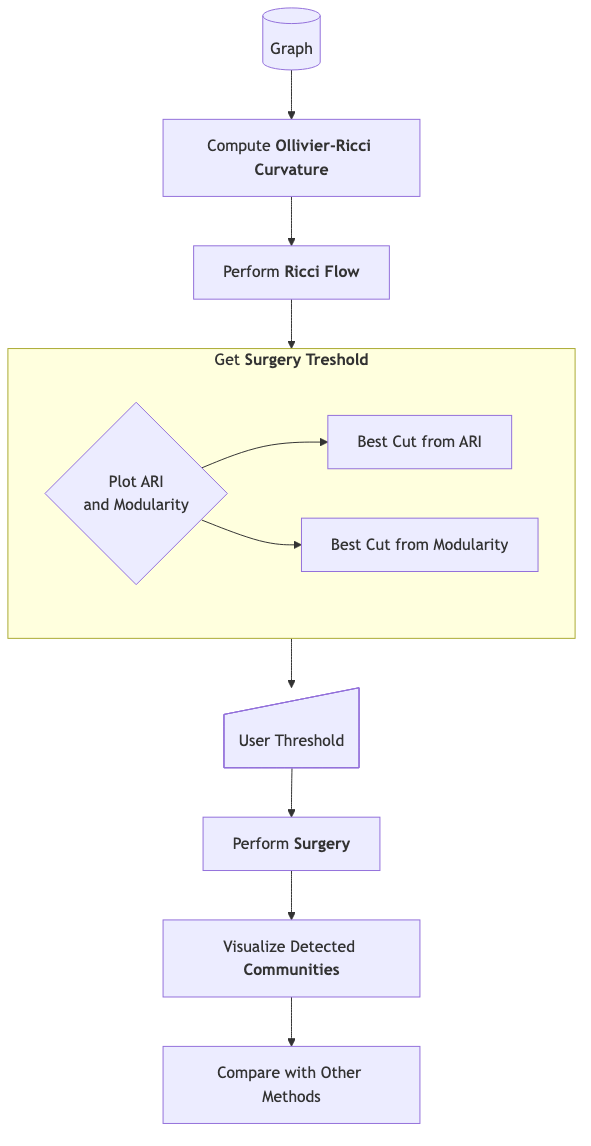
\includegraphics[width=0.7\textwidth]{Images/workflow.png}
    \caption{Code workflow.}
\end{figure}\label{fig:workflow}
